\chapter{Conceptual Model}

Users will navigate to our application on an iPad tablet in order to use the system. Upon launching the app, they will be greeted with the keyboard view, as shown in Figure~\ref{fig:ui}, which they can immediately start using to type what they want to communicate.

\begin{figure}[htb]
\centering
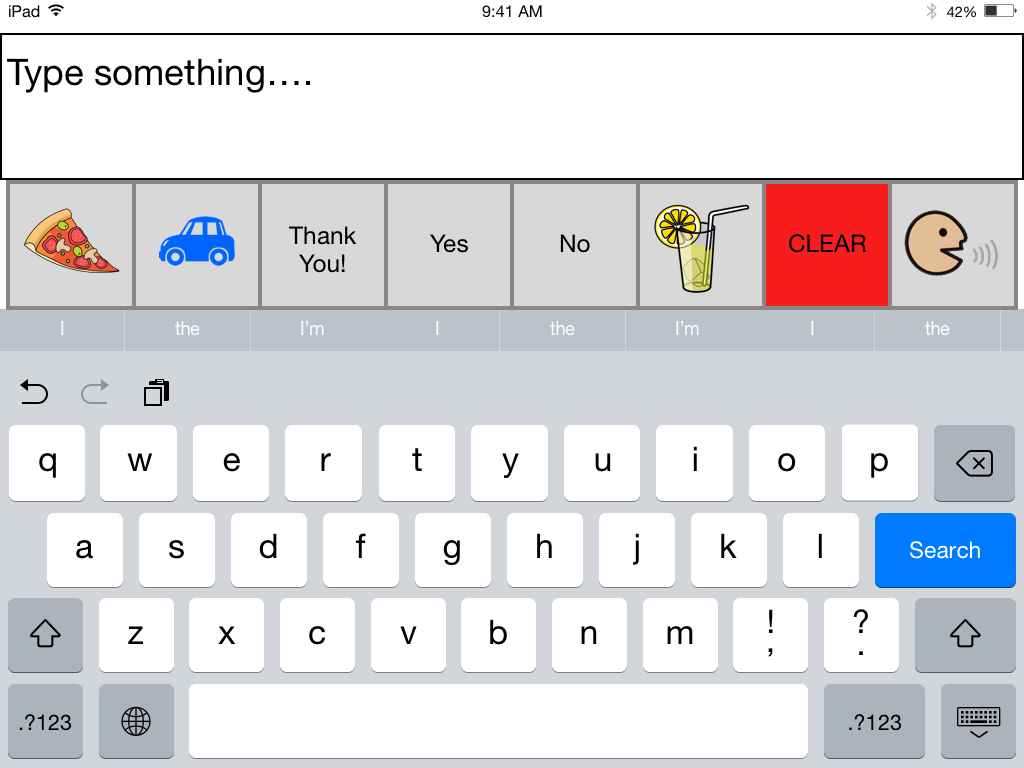
\includegraphics[width=\textwidth]{iPadLandscape.png}
\caption{Mockup of text-entry user interface}
\label{fig:ui}
\end{figure}

As they continue to type, the suggestions will adjust dynamically to both their input and any verbal feedback from the environment. The app will listen for audible speech, process the speech and prioritize the suggestions displayed to the user.  The system will first look for previous personal responses from the user to this or similar questions. After, it will display possible global responses from our database. In this way, previous personal responses will be prioritized above the global responses. This will be reflected in the application's interface as shown in Figure~\ref{fig:uiDynamic}.

\begin{figure}[htb]
\centering
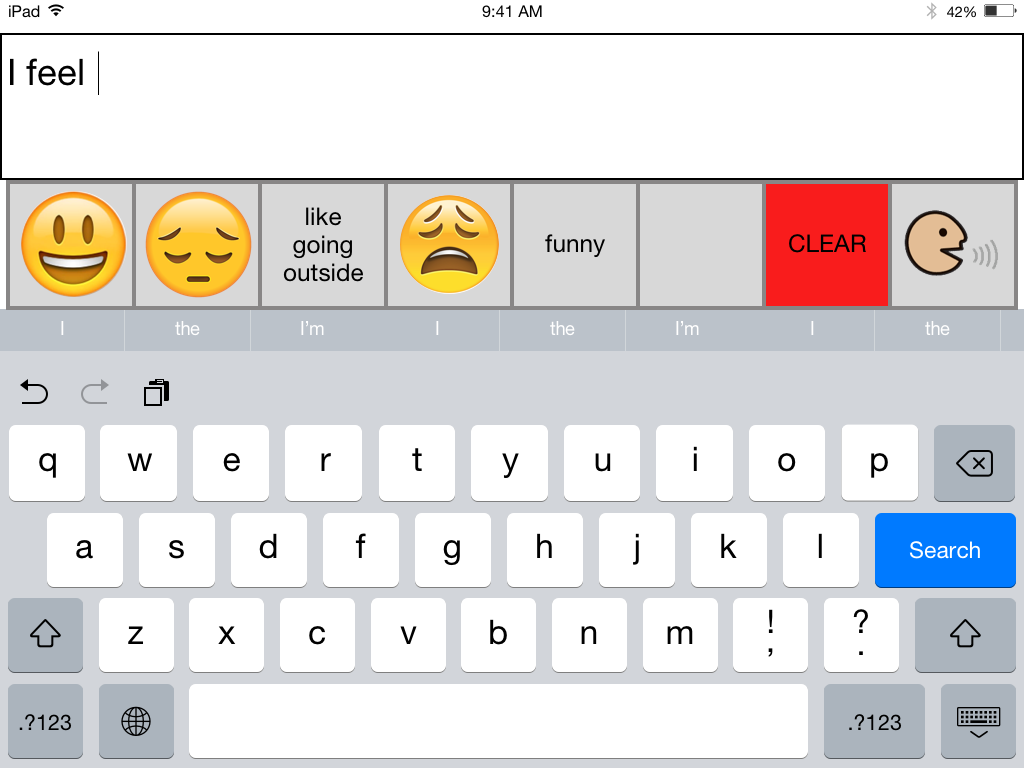
\includegraphics[width=\textwidth]{iPadLandscapeDynamic.png}
\caption{Mockup demonstrating the dynamic nature of suggestions}
\label{fig:uiDynamic}
\end{figure}

Whenever the user has completed either typing or selecting what they want to communicate, they will press the button on the right of the screen, which will speak what they have selected aloud. If the user then wants to clear the selection, they can use the clear button on the left of the speak button. This will allow the user to restart the process.
